\section{Event Selection}

\subsection{Trigger selection}
\label{sec:DiHiggs:triggers}
Events in the $\tau_\text{lep}\tau_\text{had}$ categories 
are recorded using a combination of single-lepton triggers (SLTs) 
and lepton-plus-$\tau_\text{had-vis}$ triggers (LTTs). 
The SLTs require an electron or muon to be reconstructed 
at the HLT with a minimum $E_\text{T}$ threshold that 
ranges from 24~GeV to 26~GeV for electrons and 
a minimum $p_\text{T}$ threshold that 
ranges from 20~GeV to 26~GeV for muons, 
depending on the data-taking period. 
The LTTs require that an electron with $E_\text{T}>17$~GeV 
or a muon with $p_\text{T}>14$~GeV in addition to 
a $\tau_\text{had-vis}$ with $p_\text{T}>25$~GeV are reconstructed at the HLT. 
From the 2017 data-taking period onward, 
for the LTTs that rely on an electron at the HLT or 
a $\tau_\text{had-vis}$ with a $p_\text{T}$ threshold below 35~GeV, 
either an additional jet with $E_\text{T}>25~\text{GeV}$ or 
two additional jets with $E_\text{T}>12~\text{GeV}$ are required 
at the Level-1 trigger to reduce the trigger rates. 
To ensure that the trigger reaches its efficiency plateau, 
the offline electrons, muons and $\tau_\text{had-vis}$ objects 
are required to be within $\Delta R<0.07$, $\Delta R<0.1$ 
and $\Delta R<0.2$ of the corresponding objects at the HLT, respectively. 
Minimum $p_\text{T}$ thresholds are applied to the offline objects, 
which are 1~GeV above the thresholds for electrons and muons at the HLT, 
5~GeV above the thresholds for $\tau_\text{had-vis}$ at the HLT, 
and 80~GeV (45~GeV) for jets with 
Level-1 trigger $E_\text{T}$-thresholds of 25~GeV (12~GeV). 
Events which pass the offline SLT lepton $p_\text{T}$ requirements 
are not considered for the LTT to ensure no overlap with the SLT category. 
These two categories are analysed separately.
%Events passing the $\tau_\text{lep}\tau_\text{had}$ event selection are separated in different analysis categories, depending on whether they passed the SLT or LTT selections.% If the event passes both the SLT and LTT and their corresponding offline requirements, then it is added to the SLT category, and not the LTT category.% with moderate identification requirements. Electron and muon triggers with looser identification requirements are also applied, though a more stringent $p_\text{T}$ threshold is applied.
\subsection{Event preselection}
\label{sec:DiHiggs:preselection}
Before passing the events to the MVA algorithm, they are required to pass a loose
preselection criteria, given in the following. 
Events are required to contain exactly exactly 
one electron or muon, 
an oppositely charged $\tau_\text{had-vis}$, 
and exactly two $b$-tagged jets.
The selected electron (muon) must pass a 
tight (medium) identification requirement with an efficiency of around 80\% (97\%).

% and the (sub-)leading $b$-tagged jet is required to have $p_\text{T}>45~(20)$~GeV. 
The invariant mass of the $\tau$-lepton pair ($m_{\tau\tau}^\text{MMC}$) 
is estimated from the four-momenta of the electron or muon, 
the $\tau_\text{had-vis}$ and the $\mathbf{p}_\text{T}^\text{miss}$ 
using the Missing Mass Calculator (MMC)~\cite{Elagin:2010aw}, 
which assumes that the $\mathbf{p}_\text{T}^\text{miss}$ is exclusively from the neutrinos 
produced in the $\tau$-lepton decays. 
To reject background events from low-mass Drell-Yan events, $m_{\tau\tau}^\text{MMC}$ is required to be above 60~GeV.
The $b$-tagged jet pair invariant mass ($m_{bb}$) is required to be less than 150~GeV 
to reject $t\bar t$ background events, and to allow for the definition of 
a $t\bar t$-enriched region which is used in the estimation of $t\bar t$ backgrounds, 
as described in Section~\ref{sec:DiHiggs:background}. 
A $\tau_\text{had-vis}$ with $p_\text{T}>20$~GeV and 
$\vert\eta\vert<2.3$ is required in the SLT category, 
and a $\tau_\text{had-vis}$ with $p_\text{T}>30$~GeV, 
or higher if required by the trigger, 
and $\vert\eta\vert<2.3$ is required in the LTT category. 
In both categories, the (sub-)leading $b$-tagged jet 
must have $p_\text{T}>45~(20)$~GeV, 
in addition to any trigger-dependent requirements.
The full event selection is summarised in Table~\ref{tab:DiHiggs:selectionsummary}. 

The rate of events accepted by the detector 
and selected by the analysis selection are quantified by the acceptance and the selection efficiency,
respectively.
The acceptance times efficiency for the non-resonant ggF+VBF $HH\to b\bar b\tau^+\tau^-$ signal 
is evaluated with respect to the targeted $\tau$-lepton decay modes to be 4.0\% (1.0\%) 
in the $\tau_\text{lep}\tau_\text{had}$ SLT (LTT) categories.
For the resonant $HH$ signal, the acceptance times efficiency is shown in Figure~\ref{fig:selection:acceptances} 
as a function of the resonance mass. 
The decrease in acceptance times efficiency for $m_X$ greater than about 1000~GeV 
is due to the Lorentz boost of the Higgs bosons causing their decay products to become highly collimated more often.
% The drop in acceptance times efficiency at high resonance mass is because the Higgs bosons are highly boosted, and so their decay products are collimated. This leads to loss in the reconstruction efficiency for both $\tau_\text{had-vis}$ in the $\tau_\text{had}\tau_\text{had}$ channel as the $\tau_\text{had-vis}$ begin to overlap, and to a loss in efficiency of the lepton isolation requirement in the $\tau_\text{lep}\tau_\text{had}$ channel.% This would lead to loss of acceptance times efficiency due to the lepton isolation requirement in the $\tau_\text{lep}\tau_\text{had}$) channel, and higher chance of merging of the two $\tau_\text{had}$ into one reconstructed $\tau_\text{had-vis}$ candidate for the $\tau_\text{had}\tau_\text{had}$ channel. increases with the resonance mass from 0.6\% (1.7\%) at $m_{X}=260$~GeV to 10.3\% (10\% ???) at $m_{X}=1$~TeV, but then drops to 3.6\% (3.3\% ???) at $m_{X}=1.6$~TeV in the $\tau_\text{had}\tau_\text{had}$ (combined SLT and LTT $\tau_\text{lep}\tau_\text{had}$) channel, as % The decrease in acceptance times efficiency for $m_X$ greater than about 1000~GeV is due to the Lorentz boost of the Higgs bosons decreasing the efficiencies to reconstruct and identify their decay products.

\begin{table}[!htbp]

%Events in the $\tau_\text{had}\tau_\text{had}$ trigger categories are analysed together, and events in the $\tau_\text{lep}\tau_\text{had}$ trigger categories are analysis separately.

 \centering
 \resizebox{0.72\textwidth}{!}{
 \begin{tabular}{C{0.39\textwidth}C{0.39\textwidth}}
 \toprule
 \multicolumn{2}{c}{$\tau_\text{lep}\tau_\text{had}$ categories}\\
 %% Single-$\tau_\text{had}$ trigger (STT) & Di-$\tau_\text{had}$ trigger (DTT) & Single-$e/\mu$ trigger (SLT) & $e/\mu+\tau_\text{had}$ trigger (LTT)\\
 SLT & LTT\\
 \midrule
 \multicolumn{2}{c}{\BF{$e/\mu$ selection}}\\
 \multicolumn{2}{c}{Exactly one tight $e$ or medium $\mu$}\\
 $p_\text{T}^e>25,27~\text{GeV}$ & $18~\text{GeV}<p_\text{T}^e<\text{SLT cut}$\\
 $p_\text{T}^\mu>21,27~\text{GeV}$ & $15~\text{GeV}<p_\text{T}^\mu<\text{SLT cut}$\\
 \multicolumn{2}{c}{$\vert\eta^e\vert<2.47$, not $1.37<\vert\eta^e\vert<1.52$}\\
 \multicolumn{2}{c}{$\vert\eta^\mu\vert<2.7$}\\
 \midrule
 \multicolumn{2}{c}{\BF{$\tau_\text{had-vis}$ selection}}\\
 \multicolumn{2}{c}{One loose $\tau_\text{had-vis}$}\\
 \multicolumn{2}{c}{$\vert\eta\vert<2.3$}\\
$p_\text{T}>20~\text{GeV}$ & $p_\text{T}>30~\text{GeV}$\\
 \midrule
 \multicolumn{2}{c}{\BF{Jet selection}}\\
 \multicolumn{2}{c}{$\geq 2$ jets with $\vert\eta\vert<2.5$}\\
 $p_\text{T}>45~(20)~\text{GeV}$ & Trigger dependent\\
 \midrule
 \multicolumn{2}{c}{\BF{Event-level selection}}\\
 \multicolumn{2}{c}{Trigger requirements passed}\\
 \multicolumn{2}{c}{Collision vertex reconstructed}\\
 \multicolumn{2}{c}{$m_{\tau\tau}^\text{MMC}>60~\text{GeV}$}\\
 \multicolumn{2}{c}{Opposite-sign electric charges of $e/\mu/\tau_\text{had-vis}$ and $\tau_\text{had-vis}$}\\
 \multicolumn{2}{c}{Exactly two $b$-tagged jets}\\
 %% \multicolumn{4}{c}{$b$-tagged jet $p_\text{T}>45~(20)~\text{GeV}$}\\
\multicolumn{2}{c}{$m_{bb}<150~\text{GeV}$}\\
 \bottomrule
 \end{tabular}
 }
 \caption{Summary of the event selections, 
 shown separately for the SLT and LTT. 
In cases where pairs of reconstructed objects of the same type are required, 
thresholds on the (sub-)leading $p_\text{T}$ object are given 
outside (within) parentheses. 
When the selection depends on the year of data-taking, 
the possible values of the requirements are separated by commas, 
except for the jet selection in the 
LTT channel which use multiple selection criteria as described 
in Section~\ref{sec:DiHiggs:triggers}. 
The trigger $p_\text{T}$ thresholds shown correspond to the offline requirements.}
\label{tab:DiHiggs:selectionsummary}
\end{table}

\begin{figure}[!htbp]
\centering
\includegraphics[width=0.85\linewidth]{DiHiggs/plots/acc_eff.png}
% location:/hepstore/zhiyuan/Code_latest/test, run  python ../plotcasual.py to get
\caption{Acceptance times efficiency for the \lephad\ selection 
as a function of the resonance mass $m_X$ in
SLT, LTT and SLT LTT combined.
The acceptance times efficiency is evaluated 
for $X\to HH\to b\bar{b}\tau^+\tau^-$ decays, 
with respect to the targeted \lephad\ decay mode.}
\label{fig:selection:acceptances}
\end{figure}

\subsection{Multivariate signal extraction}
\label{sec:DiHiggs:MVA}

% Multivariate discriminants (MVAs) evaluated on events 
% passing the above selections are used to extract possible signals. 
% Parameterised neural networks (PNNs) are used 
% in the search for resonant $HH$ production, and neural networks (NNs) 
% are used in the search for non-resonant $HH$. 

% During training, the sum of all backgrounds normalised to
% their respective cross-sections is used. 
% The backgrounds containing fake-$\tau_\text{had-vis}$ 
% are modelled using MC simulation. 
% The PNNs are parameterised in the mass of the heavy resonance, 
% providing near-optimal sensitivity and continuity over 
% the range of signal masses considered. 
% The hyperparameters were optimised separately for each MVA 
% using a random scan followed by a Bayesian optimisation procedure. 
% % The 375~GeV resonant $HH$ signal is not used in the PNN trainings. 
% %Additionally, the PNNs interpolate well between the mass points used for the training.% The background does not have a well defined value of the heavy resonance or LQ mass, so during training the background events are assigned a random value from the signal parameter values. Maybe mention that NNs are optimal / sufficient statistic?. , where a single binary classifier is not optimal for all signal masses. without major loss of sensitivity, allowing results to be quoted for masses other than those used during training


The di-Higgs non-resonant SM signal is well-defined in its kinematic properties, and so a 
neural network trained on this signal is used in the \lephad\ channel.
The di-Higgs resonant signal, however, is not a single signal hypothesis, 
but rather a set of continuous signal hypotheses parameterised by 
the mass of the heavy resonance which decays to Higgs boson pairs.
For these cases, a standard binary classification algorithm is not optimal. 
A set of single discriminants trained on each of the simulated signal hypotheses 
would provide good discrimination for the simulated hypotheses, 
but can not interpolate well between these points. 
For this reason, and to reduce the number of algorithms that require training, 
Parametric Neural Networks (PNNs)~\cite{Baldi:2016fzo} are used 
for the extraction of the resonant signal. PNNs are neural networks 
which enable optimal signal-to-background classification
for signal spectra connected by one or more physics parameters. 
As this problem is a smoothly-varying learning task, 
the PNN is not just able to learn how to classify signals at the simulated signal mass training
points, but also how to interpolate between them. 
Figure~\ref{fig:MVA:mass-response} shows the PNN response 
in terms of Asimov significance as a function of the PNN mass
parameter obtained for signal samples with different masses. 
This is showing the mass resolution of the PNN.

The (P)NNs are trained using Keras~\cite{chollet2015keras} 
with the Tensorflow~\cite{tensorflow2015-whitepaper} backend. 
The PNNs used in the analyses described in this note take as an input parameter to specify which signal
should be targeted, along side the feature variables, the heavy resonance mass for the di-Higgs analysis.
During training, the PNNs are trained on all the signals simultaneously, and are provided with the
generator-level masses of the signals and a random mass from the distribution of simulated signal masses
for the background. The background events are provided with such distribution of simulated signal masses
because the background events do not have a well-defined value for the ``truth scalar resonance mass'' and
the `parameter' assigned to background events must be uninformative regarding the signal / background
discrimination. This is achieved by randomly assigning a ``truth scalar resonance mass'' that follows the
distribution seen in the signal training events. During implementation, the mass of the targeted signal
is given, which results in optimal discrimination for that signal hypothesis. As the ideal neural network
output (when trained on the binary cross entropy) is a monotonic function of the signal-to-background
density ratio, this means that the PNN will optimally classify the targeted signal events, as specified by the
physics input parameter.

%% Neural network (NN) and parameterised neural network (PNN)~\cite{Baldi:2016fzo} outputs applied to events passing the above selections are used to extract possible signals for the non-resonant and resonant search, respectively. During the training of the (P)NNs, the sum of all backgrounds weighted by their cross-sections are used in the $HH$ search, and the dominant $t\bar t$ background is used in LQ search. The PNN is parameterised in the mass of the heavy resonance (LQ) for the $HH$ (LQ) search, providing near-optimal sensitivity over the range of signal masses considered, and interpolates well between the mass points used for training.% The background does not have a well defined value of the heavy resonance or LQ mass, so during training the background events are assigned a random value from the signal parameter values. Maybe mention that NNs are optimal / sufficient statistic?. , where a single binary classifier is not optimal for all signal masses. without major loss of sensitivity, allowing results to be quoted for masses other than those used during training

The same choice of MVA input variables is used for the resonant and non-resonant production modes, though different input variables are used in the different analysis categories. These variables are listed in Table~\ref{tab:selection:mvas:HHinputs}, and are defined as follows:
\begin{itemize}
\item $m_{HH}$ is the invariant mass of the $HH$ system as reconstructed from the $\tau$-lepton pair (calculated using the MMC) and the $b$-tagged jet pair;
\item $\Delta R(\tau, \tau)$ is evaluated between the two $\tau_\text{had-vis}$ (the electron or muon and the $\tau_\text{had-vis}$) in the $\tau_\text{had}\tau_\text{had}$ category ($\tau_\text{lep}\tau_\text{had}$ categories);
\item $\Delta R(b, b)$ is evaluated between the $b$-tagged jets;
\item $\Delta p_\text{T}(\ell, \tau)$ is the difference between the transverse momenta of the lepton and the $\tau_\text{had-vis}$;
\item $m_\text{T}^W =\sqrt{2p_\text{T}^\ell E_\text{T}^\text{miss}(1-\cos\Delta\phi_{\ell,\mathbf{p}_\text{T}^\text{miss}})}$ is the transverse mass of the lepton and the $\mathbf{p}_\text{T}^\text{miss}$;

\item the $\mathbf{p}_\text{T}^\text{miss}~\phi$ centrality specifies the angular position of the $\mathbf{p}_\text{T}^{\text{miss}}$ relative to the $\tau_\text{had-vis}$ in the transverse plane~\cite{HIGG-2013-32} and is defined as $(A+B)/\sqrt{A^2+B^2}$, where $A=\sin(\phi_{\mathbf{p}_\text{T}^\text{miss}}-\phi_{\tau_2})/\sin(\phi_{\tau_1}-\phi_{\tau_2})$, $B=\sin(\phi_{\tau_1}-\phi_{\mathrm{p}_\text{T}^\text{miss}})/\sin(\phi_{\tau_1}-\phi_{\tau_2})$, and $\tau_1$ and $\tau_2$ represent the two $\tau_\text{had-vis}$ (electron or muon and $\tau_\text{had-vis}$) in the case of the $\tau_\text{had}\tau_\text{had}$ category ($\tau_\text{lep}\tau_\text{had}$ categories);

\item $\Delta\phi(\ell\tau, bb)$ is the azimuthal angle between the $\ell+\tau_\text{had-vis}$ system and the $b$-tagged jet pair;
\item $\Delta\phi(\ell, \mathbf{p}_\text{T}^\text{miss})$ is the azimuthal angle between the lepton and the $\mathbf{p}_\text{T}^\text{miss}$;
\item $\Delta\phi(\ell\tau, \mathbf{p}_\text{T}^\text{miss})$ is the azimuthal angle between the electron or muon and $\tau_\text{had-vis}$ system and the $\mathbf{p}_\text{T}^\text{miss}$;
\item $S_\text{T}$ is the total transverse energy in the event, summed over all jets, $\tau_\text{had-vis}$ and leptons in the event and $E_\text{T}^\text{miss}$.%sum of hadronic energy in the event transverse to the beamline;
\end{itemize}
%% Signal events tend to have a lower $m_\text{T}^W$ than the $t\bar t$ process because the transverse mass of a lepton and neutrino decaying from a $W$~boson in a $t\bar t$ event tends to peak at $m_W\approx 80~\text{GeV}$.
The $m_{HH}$, $m_{\tau\tau}^\text{MMC}$ and $m_{bb}$ distributions are shown 
in Figure~\ref{fig:selection:mvas:mHHmMMCmbb}. 
For all categories of the non-resonant search, 
$m_{\tau\tau}^\text{MMC}$ and $m_{bb}$ are among 
the three most important MVA input variables. 
For the resonant search, five values of $m_X$ were tested in all categories, 
and $m_{HH}$ was found to be the most important MVA input variable in all cases 
except for at lower values of $m_X$ in the $\tau_\text{had}\tau_\text{had}$ category.

\begin{table}[!htbp]
\caption{Variables used as inputs to the MVAs in the three analysis categories. The same choice of input variables is used for the resonant and non-resonant production modes. The variables are defined in the main text.}
\label{tab:selection:mvas:HHinputs}
 \centering
 \begin{tabular}{lccc}
 \toprule
 Variable & $\tau_\text{had}\tau_\text{had}$ & $\tau_\text{lep}\tau_\text{had}$ SLT & $\tau_\text{lep}\tau_\text{had}$ LTT\\
 \midrule
 $m_{HH}$ & \ding{51} & \ding{51} & \ding{51} \\
 $m_{\tau\tau}^\text{MMC}$ & \ding{51} & \ding{51} & \ding{51} \\
 $m_{bb}$ & \ding{51} & \ding{51} & \ding{51} \\
 $\Delta R(\tau, \tau)$ & \ding{51} & \ding{51} & \ding{51} \\
 $\Delta R(b, b)$ & \ding{51} & \ding{51} & \\
 $\Delta p_\text{T}(\ell, \tau)$ & & \ding{51} & \ding{51} \\
 Sub-leading $b$-tagged jet $p_\text{T}$ & & \ding{51} & \\
 $m_\text{T}^W$ & & \ding{51} & \\
 $E_\text{T}^\text{miss}$ & & \ding{51} & \\
 $\mathbf{p}_\text{T}^\text{miss}~\phi$ centrality & & \ding{51} & \\
 $\Delta\phi(\ell\tau, bb)$ & & \ding{51} & \\
 $\Delta\phi(\ell, \mathbf{p}_\text{T}^\text{miss})$ & & & \ding{51} \\
 $\Delta\phi(\ell\tau, \mathbf{p}_\text{T}^\text{miss})$ & & & \ding{51} \\
 $S_\text{T}$ & & & \ding{51} \\
 \bottomrule
 \end{tabular}
\end{table}


% \begin{figure}[!htbp]
% \centering
% \subfigure[]{\includegraphics[width=0.32\textwidth]{figures/MVAInputs/mHHPlotsIncludingResonantSignals/Region_BMin0_incJet1_distmHH_J2_Y2015_DLLOS_T2_SpcTauHH_L0_GlobalFit_conditionnal_mu0_logy.pdf}}
% \subfigure[]{\includegraphics[width=0.32\textwidth]{figures/MVAInputs/mHHPlotsIncludingResonantSignals/Region_BMin0_incJet1_distMhh_J2_DSM_T2_SpcTauLH_Y2015_LTT0_L1_GlobalFit_conditionnal_mu0_logy.pdf}}
% \subfigure[]{\includegraphics[width=0.32\textwidth]{figures/MVAInputs/mHHPlotsIncludingResonantSignals/Region_BMin0_incJet1_distMhh_J2_DSM_T2_SpcTauLH_Y2015_LTT1_L1_GlobalFit_conditionnal_mu0_logy.pdf}}\\
% \subfigure[]{\includegraphics[width=0.32\textwidth]{figures/MVAInputs/hadhad2/Region_BMin0_incJet1_distmMMC_J2_Y2015_DLLOS_T2_SpcTauHH_L0_GlobalFit_conditionnal_mu0log.pdf}}
% \subfigure[]{\includegraphics[width=0.32\textwidth]{figures/MVAInputs/lephad2/Region_BMin0_incJet1_distmMMC_J2_DSM_T2_SpcTauLH_Y2015_LTT0_L1_GlobalFit_conditionnal_mu0log.pdf}}
% \subfigure[]{\includegraphics[width=0.32\textwidth]{figures/MVAInputs/lephad2/Region_BMin0_incJet1_distmMMC_J2_DSM_T2_SpcTauLH_Y2015_LTT1_L1_GlobalFit_conditionnal_mu0log.pdf}}\\
% \subfigure[]{\includegraphics[width=0.32\textwidth]{figures/MVAInputs/hadhad2/Region_BMin0_incJet1_distmBB_J2_Y2015_DLLOS_T2_SpcTauHH_L0_GlobalFit_conditionnal_mu0log.pdf}}
% \subfigure[]{\includegraphics[width=0.32\textwidth]{figures/MVAInputs/lephad2/Region_BMin0_incJet1_distmbb_J2_DSM_T2_SpcTauLH_Y2015_LTT0_L1_GlobalFit_conditionnal_mu0log.pdf}}
% \subfigure[]{\includegraphics[width=0.32\textwidth]{figures/MVAInputs/lephad2/Region_BMin0_incJet1_distmbb_J2_DSM_T2_SpcTauLH_Y2015_LTT1_L1_GlobalFit_conditionnal_mu0log.pdf}}
% %%% \caption{Signal (solid line), post-fit backgrounds (filled histograms) and data (dots with error bars) distributions of $m_{HH}$ (above), $m_{\tau\tau}^\text{MMC}$ (middle row) and $m_{bb}$ (bottom) for events in the $\tau_\text{had}\tau_\text{had}$ channel (left), and the single-lepton trigger (middle column) and lepton-plus-$\tau_\text{had-vis}$ trigger (right) categories of the $\tau_\text{lep}\tau_\text{had}$ channel. The signal normalisation is set to the observed 95\% confidence-level limit obtained from the combined fit. The normalisation and shape of the backgrounds and the uncertainty on the total background are shown as derived from the likelihood fit to data. The uncertainty band includes statistical and systematics uncertainties on the total background. \TODO{change lephad plots to latest post-fit plots.}}
% \caption{Signal (solid lines), post-fit background (filled histograms) and data (dots with error bars) distributions of $m_{HH}$ (top), $m_{\tau\tau}^\text{MMC}$ (middle row) and $m_{bb}$ (bottom) for events in the $\tau_\text{had}\tau_\text{had}$ (left), $\tau_\text{lep}\tau_\text{had}$ single-lepton trigger (middle column) and $\tau_\text{lep}\tau_\text{had}$ lepton-plus-$\tau_\text{had-vis}$ trigger (right) categories. The normalisation and shape of the backgrounds and the uncertainty on the total background shown are determined from the likelihood fit to data in the non-resonant $HH$ search. The expected non-resonant signal is overlaid with its normalisation scaled by a factor of 100, and the $m_X=500~\text{GeV}$ and $m_X=1000~\text{GeV}$ resonant signals are overlaid in the $m_{HH}$ distributions with their cross-section set to 1~pb.
% The dashed histogram shows the total pre-fit background.
% The size of the combined statistical and systematic uncertainty of the background is indicated by the hatched band.
% The ratio of the data to the sum of the backgrounds is shown in the lower panels.}
% %% The uncertainty band includes statistical and systematic uncertainties on the total background.}
% \label{fig:selection:mvas:mHHmMMCmbb}
% \end{figure}

The (P)NNs use rectified linear unit and sigmoidal activation functions 
for the hidden and output layers, respectively, binary cross entropy as the loss function, 
and stochastic (mini-batch) gradient descent as the optimiser~\cite{Goodfellow-et-al-2016}. 
% For the PNN used in the $\tau_\text{had}\tau_\text{had}$ category, 3 layers of 128 hidden nodes, 
% followed by 1 hidden layer of 16 nodes are used. 
For the (P)NN used in the $\tau_\text{lep}\tau_\text{had}$ SLT category, 
2 layers of 512 hidden nodes are used, 
and for the (P)NN used in the $\tau_\text{lep}\tau_\text{had}$ LTT category 
3 layers of 512 (256) nodes are used. 
The (P)NN input variables are standardised by subtracting 
the median value and dividing by the interquartile range. 
Nesterov momentum and learning rate decay were used in the training of all (P)NNs, 
and in the $\tau_\text{lep}\tau_\text{had}$ categories they used an L2 regularisation term 
in the loss function~\cite{Goodfellow-et-al-2016}. 
% The BDT uses 1500 trees with a maximum depth of 2 and a 
% minimum node size of 1\% of the training events. 
% Gradient boosting is used with a shrinkage of 0.2.% The PNN used in the $\tau_\text{had}\tau_\text{had}$ category has three hidden layers of 128 nodes followed by one of 16 nodes, and the $\tau_\text{lep}\tau_\text{had}$ (P)NNs have two hidden layers of 512 nodes in the SLT category, and three hidden layers of (256) 512 nodes in the LTT category.

\begin{figure}[!htbp]
    \centering
    \includegraphics[width=0.85\linewidth]{DiHiggs/plots/mass_response.png}
    % location /hepstore/zhiyuan/Code_latest/run_Asimov/parametricnet/scripts/plots, run  python plot_mass.py to get
    \caption{
        PNN response in terms of Asimov significance as a function of the PNN mass parameter obtained for
signal samples with different masses for the di-Higgs \lephad\ channel. Due to a large difference in acceptance times
efficiency of the \lephad\ channel signal region selection depending on the mass of the resonance, 
all significances are scaled so that the maximum significance is 1 for better visibility.}
    \label{fig:MVA:mass-response}
    \end{figure}

\subsection{$Z+\text{HF}$ control region}
\label{sec:selection:zcr}

The normalisation of the $Z+\text{HF}$ background is determined 
from data by fitting the $m_{\ell\ell}$ distribution in the  a dedicated control region 
($Z+\text{HF}$ CR) in the likelihood fit. 
This is to account for a known discrepancy in the $Z+\text{HF}$ production
cross-section at NLO with respect to data, as provided for these processes in \textsc{Sherpa}. 
The $Z+\text{HF}$ CR targets events containing $Z$~boson decays to electron or muon pairs 
using triggers that require single leptons, or pairs of same-flavour leptons. 
Exactly two oppositely-charged same-flavour leptons and exactly two $b$-tagged jets are required 
to be reconstructed offline. The leptons are required to have $p_\text{T}>9~\text{GeV}$, 
pass offline $p_\text{T}$ thresholds based on the trigger thesholds, 
be compatible with originating from the primary vertex, 
and pass medium identification and loose isolation requirements. 
Lastly, the invariant mass of the lepton pair is required to be between 75~\GeV\ 
and 110~\GeV\ to select events originating from a $Z$~boson decay, 
and $m_{bb}$ is required to be less than 40~\GeV\ or greater than 210~\GeV\ 
to ensure orthogonality to other analyses containing Higgs boson decays. 
This region also provides constraints on the normalisation of the $t\bar t$ background. 
% Figure~\ref{fig:zcr} shows the post-fit background and data $m_{\ell\ell}$ distributions 
% in the $Z+\text{HF}$ control region.
% Since the branching ratios of $Z$~bosons to electrons and muons are known accurately, 
% this production cross-section is determined simultaneously using $Z\to ee$ and $Z\to\mu\mu$ events. 
% These triggers have lower $E_\text{T}$ ($p_\text{T}$) thresholds for electrons (muons) which vary with data-taking year. The corresponding offline trigger thresholds start at 25~GeV (21~GeV) for the single electron (muon) triggers, 13~GeV and 13~GeV (19~GeV and 10~GeV) for the leading and subleading lepton respectively for the di-electron (di-muon) triggers, and electron (muon) thresholds of 18~GeV (15~GeV) or 26~GeV (9~GeV) for the electron-plus-muon triggers.


% \begin{figure}[!htbp]
% \centering
% %% \subfigure[]{\includegraphics[width=0.49\textwidth]{figures/auxiliary/}}
% %% \subfigure[]{\includegraphics[width=0.95\textwidth]{figures/auxiliary/ZHF_mll.png}}
% \subfigure[]{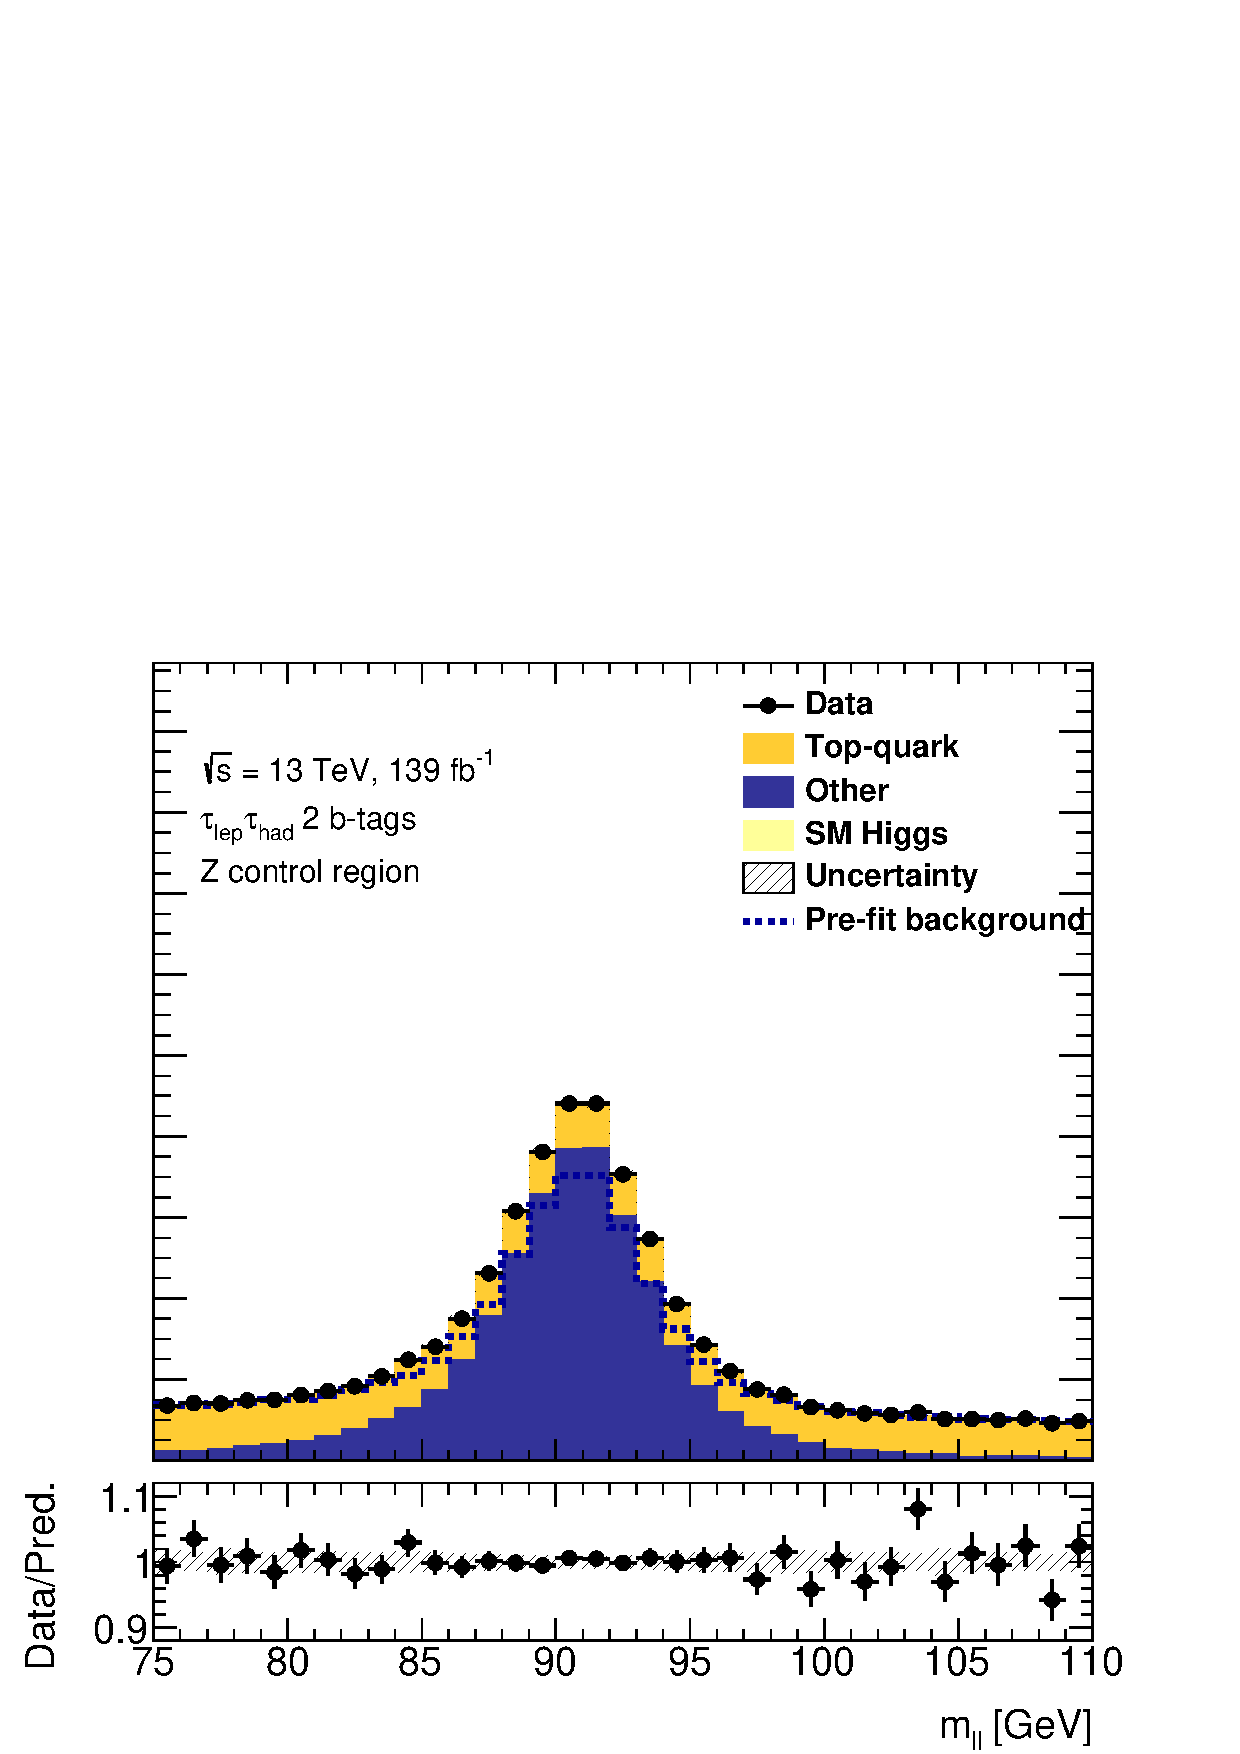
\includegraphics[width=0.50\textwidth]{figures/PostfitPlots/Region_BMin0_incJet1_Y2015_DZllbbCR_T2_L2_distmLL_J2_GlobalFit_conditionnal_mu0.pdf}}
% %%% \caption{(a) Pre-fit background and data and (b) post-fit background and data $m_{\ell\ell}$ distributions in the $Z+\text{HF}$ control region. In (b), the normalisation and shape of the backgrounds and the uncertainty on the total background are shown as determined from the likelihood fit to data in the non-resonant $HH$ search. The uncertainty band includes statistical and systematics uncertainties on the total background. \TODO{change to up-to-date plots.}}
% \caption{Post-fit background and data $m_{\ell\ell}$ distributions in the $Z+\text{HF}$ control region. The normalisation and shape of the backgrounds and the uncertainty on the total background are shown as determined from the likelihood fit to data in the non-resonant $HH$ search. The uncertainty band includes statistical and systematics uncertainties on the total background. The dashed histogram shows the total pre-fit background.}
% \label{fig:zcr}
% \end{figure}
